\documentclass[tikz, border=6pt]{standalone}
\IfFileExists{lmodern.sty}{\usepackage[T1]{fontenc}\usepackage{lmodern}}{}
\usepackage{amsmath,amssymb,bm}
\usepackage[scaled=0.95]{helvet}
\usetikzlibrary{arrows.meta, fit}
\definecolor{Blue}{HTML}{3A76D8}
\definecolor{Green}{HTML}{3BA55C}
\definecolor{Orange}{HTML}{EE8133}
\definecolor{Gray}{HTML}{6B7280}
\definecolor{Ink}{HTML}{1F2937}
\tikzset{
  tree node/.style={/utils/exec={\colorlet{pytikzarg}{#1}}, rounded corners=3pt, minimum height=6.5mm, inner sep=4pt, align=center, draw=pytikzarg!78!black, fill=pytikzarg!18, line width=0.7pt, font=\small},
  tree node/.default=Blue,
  tree edge/.style={Ink!60, line width=0.7pt},
  tree label/.style={font=\footnotesize, fill=white, inner sep=1.5pt},
}
\begin{document}
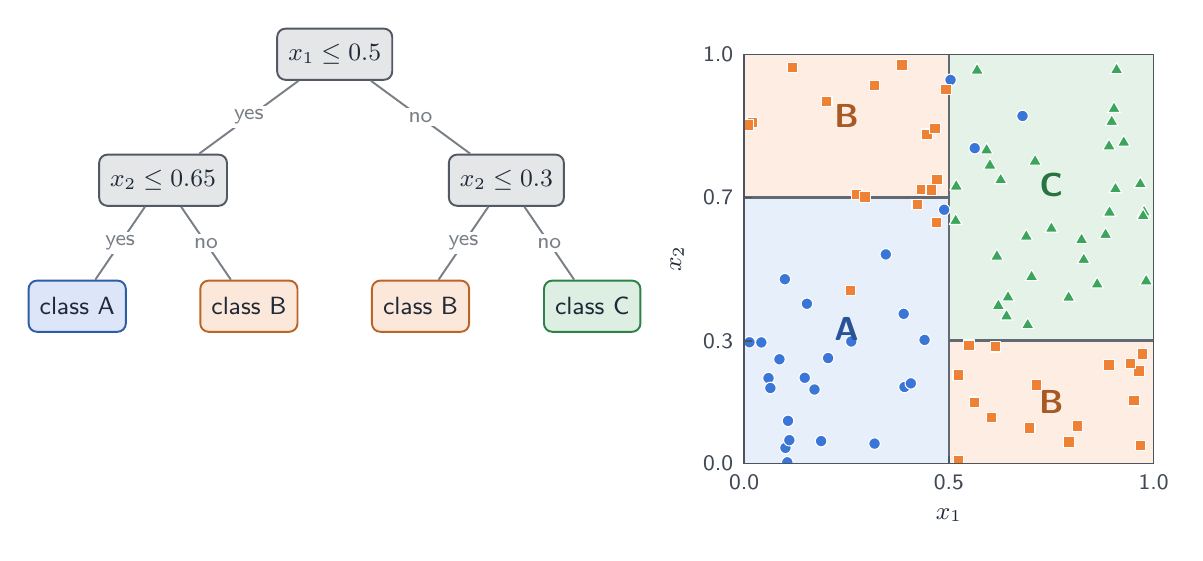
\begin{tikzpicture}[color=Ink, execute at begin picture={\sffamily}, line width=0.6pt, >={Stealth[length=5.5pt, width=4pt, inset=1.2pt]}, line join=round]
  % tree t
  \node[tree node=Gray] (t-0) at (0,2.2) {$x_1 \le 0.5$};
  \node[tree node=Gray] (t-1) at (-2.18,0.6) {$x_2 \le 0.65$};
  \node[tree node=Blue] (t-2) at (-3.27,-1) {class A};
  \node[tree node=Orange] (t-3) at (-1.09,-1) {class B};
  \node[tree node=Gray] (t-4) at (2.18,0.6) {$x_2 \le 0.3$};
  \node[tree node=Orange] (t-5) at (1.09,-1) {class B};
  \node[tree node=Green] (t-6) at (3.27,-1) {class C};
  \draw[tree edge] (t-0) -- node[tree label, midway, align=center] {yes} (t-1);
  \draw[tree edge] (t-0) -- node[tree label, midway, align=center] {no} (t-4);
  \draw[tree edge] (t-1) -- node[tree label, midway, align=center] {yes} (t-2);
  \draw[tree edge] (t-1) -- node[tree label, midway, align=center] {no} (t-3);
  \draw[tree edge] (t-4) -- node[tree label, midway, align=center] {yes} (t-5);
  \draw[tree edge] (t-4) -- node[tree label, midway, align=center] {no} (t-6);
  % axes ax1
  \begin{scope}
    \clip (5.2,-3) rectangle (10.4,2.2);
    \begin{scope}
      \clip (5.2,-3) rectangle (10.4,2.2);
      \fill[Blue!12, even odd rule] (5.2,-3) -- (5.2,0.384) -- (7.787,0.384) -- (7.8,0.371) -- (7.8,-3) --
          cycle;
      \fill[Orange!14, even odd rule] (7.813,-3) -- (7.8,-3) -- (7.8,-1.458) -- (7.813,-1.445) --
          (10.4,-1.445) -- (10.4,-3) -- cycle (5.2,0.384) -- (5.2,2.2) -- (7.8,2.2) -- (7.8,0.397) --
          (7.787,0.384) -- cycle;
      \fill[Green!14, even odd rule] (7.813,-1.445) -- (7.8,-1.432) -- (7.8,2.2) -- (10.4,2.2) --
          (10.4,-1.445) -- cycle;
    \end{scope}
    \draw[color=Ink!70, line width=1pt] (7.8,-3) -- (7.8,2.2);
    \draw[color=Ink!70, line width=1pt] (5.2,0.38) -- (7.8,0.38);
    \draw[color=Ink!70, line width=1pt] (7.8,-1.44) -- (10.4,-1.44);
    \filldraw[fill=Blue, draw=white, line width=0.4pt] (6.56,-1.448) circle[radius=2.1pt];
    \filldraw[fill=Blue, draw=white, line width=0.4pt] (6.177,-2.713) circle[radius=2.1pt];
    \filldraw[fill=Blue, draw=white, line width=0.4pt] (7.236,-2.026) circle[radius=2.1pt];
    \filldraw[fill=Blue, draw=white, line width=0.4pt] (6.999,-0.342) circle[radius=2.1pt];
    \filldraw[fill=Blue, draw=white, line width=0.4pt] (5.757,-2.456) circle[radius=2.1pt];
    \filldraw[fill=Blue, draw=white, line width=0.4pt] (8.735,1.416) circle[radius=2.1pt];
    \filldraw[fill=Blue, draw=white, line width=0.4pt] (5.724,-2.799) circle[radius=2.1pt];
    \filldraw[fill=Blue, draw=white, line width=0.4pt] (7.317,-1.98) circle[radius=2.1pt];
    \filldraw[fill=Blue, draw=white, line width=0.4pt] (6.093,-2.058) circle[radius=2.1pt];
    \filldraw[fill=Blue, draw=white, line width=0.4pt] (5.717,-0.657) circle[radius=2.1pt];
    \filldraw[fill=Blue, draw=white, line width=0.4pt] (7.74,0.225) circle[radius=2.1pt];
    \filldraw[fill=Blue, draw=white, line width=0.4pt] (7.821,1.874) circle[radius=2.1pt];
    \filldraw[fill=Blue, draw=white, line width=0.4pt] (5.418,-1.46) circle[radius=2.1pt];
    \filldraw[fill=Blue, draw=white, line width=0.4pt] (5.267,-1.458) circle[radius=2.1pt];
    \filldraw[fill=Blue, draw=white, line width=0.4pt] (5.774,-2.701) circle[radius=2.1pt];
    \filldraw[fill=Blue, draw=white, line width=0.4pt] (6.856,-2.745) circle[radius=2.1pt];
    \filldraw[fill=Blue, draw=white, line width=0.4pt] (7.226,-1.097) circle[radius=2.1pt];
    \filldraw[fill=Blue, draw=white, line width=0.4pt] (5.969,-1.909) circle[radius=2.1pt];
    \filldraw[fill=Blue, draw=white, line width=0.4pt] (7.491,-1.428) circle[radius=2.1pt];
    \filldraw[fill=Blue, draw=white, line width=0.4pt] (5.509,-1.913) circle[radius=2.1pt];
    \filldraw[fill=Blue, draw=white, line width=0.4pt] (8.128,1.007) circle[radius=2.1pt];
    \filldraw[fill=Blue, draw=white, line width=0.4pt] (5.533,-2.039) circle[radius=2.1pt];
    \filldraw[fill=Blue, draw=white, line width=0.4pt] (5.648,-1.674) circle[radius=2.1pt];
    \filldraw[fill=Blue, draw=white, line width=0.4pt] (5.748,-2.983) circle[radius=2.1pt];
    \filldraw[fill=Blue, draw=white, line width=0.4pt] (6.266,-1.659) circle[radius=2.1pt];
    \filldraw[fill=Blue, draw=white, line width=0.4pt] (5.997,-0.969) circle[radius=2.1pt];
    \filldraw[fill=Orange, draw=white, line width=0.4pt] (9.368,-2.588) rectangle (9.5,-2.456);
    \filldraw[fill=Orange, draw=white, line width=0.4pt] (6.563,0.352) rectangle (6.696,0.485);
    \filldraw[fill=Orange, draw=white, line width=0.4pt] (8.057,-2.286) rectangle (8.19,-2.153);
    \filldraw[fill=Orange, draw=white, line width=0.4pt] (7.383,0.414) rectangle (7.516,0.547);
    \filldraw[fill=Orange, draw=white, line width=0.4pt] (7.332,0.226) rectangle (7.465,0.359);
    \filldraw[fill=Orange, draw=white, line width=0.4pt] (6.788,1.74) rectangle (6.921,1.872);
    \filldraw[fill=Orange, draw=white, line width=0.4pt] (7.582,0.541) rectangle (7.715,0.674);
    \filldraw[fill=Orange, draw=white, line width=0.4pt] (6.183,1.533) rectangle (6.316,1.666);
    \filldraw[fill=Orange, draw=white, line width=0.4pt] (7.852,-1.942) rectangle (7.985,-1.809);
    \filldraw[fill=Orange, draw=white, line width=0.4pt] (7.136,1.997) rectangle (7.269,2.13);
    \filldraw[fill=Orange, draw=white, line width=0.4pt] (8.273,-2.481) rectangle (8.406,-2.348);
    \filldraw[fill=Orange, draw=white, line width=0.4pt] (5.237,1.265) rectangle (5.37,1.398);
    \filldraw[fill=Orange, draw=white, line width=0.4pt] (10.15,-1.888) rectangle (10.283,-1.755);
    \filldraw[fill=Orange, draw=white, line width=0.4pt] (5.185,1.236) rectangle (5.317,1.369);
    \filldraw[fill=Orange, draw=white, line width=0.4pt] (7.856,-3.031) rectangle (7.989,-2.898);
    \filldraw[fill=Orange, draw=white, line width=0.4pt] (8.323,-1.582) rectangle (8.456,-1.449);
    \filldraw[fill=Orange, draw=white, line width=0.4pt] (7.509,0.411) rectangle (7.641,0.544);
    \filldraw[fill=Orange, draw=white, line width=0.4pt] (9.261,-2.792) rectangle (9.394,-2.659);
    \filldraw[fill=Orange, draw=white, line width=0.4pt] (7.456,1.117) rectangle (7.589,1.25);
    \filldraw[fill=Orange, draw=white, line width=0.4pt] (10.166,-2.838) rectangle (10.298,-2.705);
    \filldraw[fill=Orange, draw=white, line width=0.4pt] (8.844,-2.065) rectangle (8.977,-1.932);
    \filldraw[fill=Orange, draw=white, line width=0.4pt] (7.987,-1.562) rectangle (8.12,-1.429);
    \filldraw[fill=Orange, draw=white, line width=0.4pt] (7.555,1.189) rectangle (7.688,1.322);
    \filldraw[fill=Orange, draw=white, line width=0.4pt] (5.745,1.966) rectangle (5.878,2.099);
    \filldraw[fill=Orange, draw=white, line width=0.4pt] (10.042,-1.794) rectangle (10.175,-1.661);
    \filldraw[fill=Orange, draw=white, line width=0.4pt] (8.76,-2.614) rectangle (8.893,-2.482);
    \filldraw[fill=Orange, draw=white, line width=0.4pt] (7.577,-0.006) rectangle (7.71,0.127);
    \filldraw[fill=Orange, draw=white, line width=0.4pt] (9.769,-1.812) rectangle (9.902,-1.679);
    \filldraw[fill=Orange, draw=white, line width=0.4pt] (10.192,-1.674) rectangle (10.325,-1.541);
    \filldraw[fill=Orange, draw=white, line width=0.4pt] (6.483,-0.869) rectangle (6.616,-0.736);
    \filldraw[fill=Orange, draw=white, line width=0.4pt] (6.67,0.319) rectangle (6.803,0.452);
    \filldraw[fill=Orange, draw=white, line width=0.4pt] (10.082,-2.268) rectangle (10.215,-2.135);
    \filldraw[fill=Orange, draw=white, line width=0.4pt] (7.698,1.685) rectangle (7.831,1.818);
    \filldraw[fill=Green, draw=white, line width=0.4pt] (8.321,0.881) -- (8.239,0.741) -- (8.402,0.741) -- cycle;
    \filldraw[fill=Green, draw=white, line width=0.4pt] (10.231,0.644) -- (10.149,0.504) -- (10.312,0.504) -- cycle;
    \filldraw[fill=Green, draw=white, line width=0.4pt] (9.834,1.125) -- (9.753,0.985) -- (9.915,0.985) -- cycle;
    \filldraw[fill=Green, draw=white, line width=0.4pt] (8.551,-0.794) -- (8.47,-0.934) -- (8.632,-0.934) -- cycle;
    \filldraw[fill=Green, draw=white, line width=0.4pt] (7.886,0.178) -- (7.805,0.038) -- (7.967,0.038) -- cycle;
    \filldraw[fill=Green, draw=white, line width=0.4pt] (9.683,-0.629) -- (9.602,-0.769) -- (9.764,-0.769) -- cycle;
    \filldraw[fill=Green, draw=white, line width=0.4pt] (9.84,0.284) -- (9.758,0.143) -- (9.921,0.143) -- cycle;
    \filldraw[fill=Green, draw=white, line width=0.4pt] (9.513,-0.318) -- (9.431,-0.458) -- (9.594,-0.458) -- cycle;
    \filldraw[fill=Green, draw=white, line width=0.4pt] (8.801,-1.145) -- (8.72,-1.285) -- (8.882,-1.285) -- cycle;
    \filldraw[fill=Green, draw=white, line width=0.4pt] (8.85,-0.534) -- (8.769,-0.675) -- (8.931,-0.675) -- cycle;
    \filldraw[fill=Green, draw=white, line width=0.4pt] (9.868,1.435) -- (9.787,1.295) -- (9.949,1.295) -- cycle;
    \filldraw[fill=Green, draw=white, line width=0.4pt] (8.279,1.075) -- (8.198,0.935) -- (8.36,0.935) -- cycle;
    \filldraw[fill=Green, draw=white, line width=0.4pt] (9.102,0.079) -- (9.021,-0.061) -- (9.183,-0.061) -- cycle;
    \filldraw[fill=Green, draw=white, line width=0.4pt] (8.41,-0.274) -- (8.329,-0.414) -- (8.491,-0.414) -- cycle;
    \filldraw[fill=Green, draw=white, line width=0.4pt] (8.783,-0.021) -- (8.702,-0.161) -- (8.864,-0.161) -- cycle;
    \filldraw[fill=Green, draw=white, line width=0.4pt] (10.021,1.172) -- (9.94,1.032) -- (10.102,1.032) -- cycle;
    \filldraw[fill=Green, draw=white, line width=0.4pt] (10.306,-0.589) -- (10.225,-0.729) -- (10.387,-0.729) -- cycle;
    \filldraw[fill=Green, draw=white, line width=0.4pt] (9.93,2.094) -- (9.849,1.954) -- (10.011,1.954) -- cycle;
    \filldraw[fill=Green, draw=white, line width=0.4pt] (9.897,1.601) -- (9.816,1.46) -- (9.978,1.46) -- cycle;
    \filldraw[fill=Green, draw=white, line width=0.4pt] (10.279,0.288) -- (10.197,0.148) -- (10.36,0.148) -- cycle;
    \filldraw[fill=Green, draw=white, line width=0.4pt] (8.428,-0.902) -- (8.347,-1.043) -- (8.509,-1.043) -- cycle;
    \filldraw[fill=Green, draw=white, line width=0.4pt] (9.485,-0.064) -- (9.404,-0.205) -- (9.566,-0.205) -- cycle;
    \filldraw[fill=Green, draw=white, line width=0.4pt] (9.321,-0.797) -- (9.24,-0.937) -- (9.402,-0.937) -- cycle;
    \filldraw[fill=Green, draw=white, line width=0.4pt] (10.267,0.239) -- (10.186,0.099) -- (10.348,0.099) -- cycle;
    \filldraw[fill=Green, draw=white, line width=0.4pt] (9.79,0.001) -- (9.709,-0.139) -- (9.871,-0.139) -- cycle;
    \filldraw[fill=Green, draw=white, line width=0.4pt] (9.916,0.581) -- (9.834,0.441) -- (9.997,0.441) -- cycle;
    \filldraw[fill=Green, draw=white, line width=0.4pt] (8.532,-1.035) -- (8.451,-1.175) -- (8.613,-1.175) -- cycle;
    \filldraw[fill=Green, draw=white, line width=0.4pt] (8.458,0.695) -- (8.376,0.555) -- (8.539,0.555) -- cycle;
    \filldraw[fill=Green, draw=white, line width=0.4pt] (8.158,2.087) -- (8.077,1.947) -- (8.239,1.947) -- cycle;
    \filldraw[fill=Green, draw=white, line width=0.4pt] (8.895,0.932) -- (8.813,0.792) -- (8.976,0.792) -- cycle;
    \filldraw[fill=Green, draw=white, line width=0.4pt] (7.893,0.616) -- (7.812,0.475) -- (7.975,0.475) -- cycle;
  \end{scope}
  \draw[Ink!80, line width=0.5pt] (5.2,-3) rectangle (10.4,2.2);
  \draw[Ink!80, line width=0.5pt] (5.2,-3) -- (5.2,-2.9) (7.8,-3) -- (7.8,-2.9) (10.4,-3) --
      (10.4,-2.9) (5.2,-3) -- (5.3,-3) (5.2,-1.44) -- (5.3,-1.44) (5.2,0.38) -- (5.3,0.38) (5.2,2.2)
      -- (5.3,2.2);
  \node[anchor=north, font=\footnotesize, text=Ink!85, inner sep=2pt] (ax1-xt0) at (5.2,-3.06) {0.0};
  \node[anchor=north, font=\footnotesize, text=Ink!85, inner sep=2pt] (ax1-xt1) at (7.8,-3.06) {0.5};
  \node[anchor=north, font=\footnotesize, text=Ink!85, inner sep=2pt] (ax1-xt2) at (10.4,-3.06) {1.0};
  \node[anchor=east, font=\footnotesize, text=Ink!85, inner sep=2pt] (ax1-yt0) at (5.14,-3) {0.0};
  \node[anchor=east, font=\footnotesize, text=Ink!85, inner sep=2pt] (ax1-yt1) at (5.14,-1.44) {0.3};
  \node[anchor=east, font=\footnotesize, text=Ink!85, inner sep=2pt] (ax1-yt2) at (5.14,0.38) {0.7};
  \node[anchor=east, font=\footnotesize, text=Ink!85, inner sep=2pt] (ax1-yt3) at (5.14,2.2) {1.0};
  \node[text=Blue!70!black, font=\large] at (6.5,-1.284) {\textbf{A}};
  \node[text=Orange!70!black, font=\large] at (6.5,1.42) {\textbf{B}};
  \node[text=Orange!70!black, font=\large] at (9.1,-2.22) {\textbf{B}};
  \node[text=Green!70!black, font=\large] at (9.1,0.536) {\textbf{C}};
  \node[fit=(ax1-xt0)(ax1-xt1)(ax1-xt2), inner sep=0pt] (ax1-xticks) {};
  \node[anchor=north, font=\small, align=center, inner sep=4pt] at (7.8,0 |- ax1-xticks.south) {$x_1$};
  \node[fit=(ax1-yt0)(ax1-yt1)(ax1-yt2)(ax1-yt3), inner sep=0pt] (ax1-yticks) {};
  \node[anchor=south, rotate=90, font=\small, align=center, inner sep=4pt] at (ax1-yticks.west |- 0,-0.4) {$x_2$};
\end{tikzpicture}
\end{document}
